\documentclass[conference]{IEEEtran}
\IEEEoverridecommandlockouts

\usepackage{cite}
\usepackage{amsmath,amssymb,amsfonts}
\usepackage{graphicx}
\usepackage{textcomp}
\usepackage{xcolor}
\usepackage{booktabs}
\usepackage[T1]{fontenc}
\usepackage{lmodern}

\begin{document}

\title{Energy Cost of Streaming Delivery and Security Choices:\\
An Empirical Study of Protocol, Codec, and DRM Effects}

\author{
\IEEEauthorblockN{Hassaan Ali}
\IEEEauthorblockA{
  \textit{Department of Computer Science}\\
  \textit{The University of Texas at Austin}\\
  Austin, TX, USA\\
  hassaaniali@utexas.edu}
\and
\IEEEauthorblockN{Shyamal Gupta}
\IEEEauthorblockA{
  \textit{Department of Computer Science}\\
  \textit{The University of Texas at Austin}\\
  Austin, TX, USA\\
  shyamal.gupta@utexas.edu}
}

\maketitle

\begin{abstract}
Video streaming dominates downstream internet traffic, so delivery and security design
choices directly influence client energy use. This paper presents a controlled empirical
study of client-side streaming energy across two experiment suites. The first suite
compares HLS over HTTP/1.1 and HTTP/2, with TLS and AES-128 toggles, under 30 trials.
The second suite adds codec and DRM-style comparisons under 50 additional trials,
including rate-limited bulk transfer (MP4, MKV, AV1), HLS codec variants (H.264/TS vs.
AV1/fMP4), and decryption modes that approximate AES-128-CBC, CENC-CTR, and CBCS-CBC.
Using a macOS testbed with \texttt{powermetrics}, we observe that HTTP/2 remains more
energy intensive than HTTP/1.1 for sequential HLS requests in loopback conditions, AV1
fMP4 HLS is lower energy per megabyte than H.264/TS HLS in our setup, and measured DRM
mode differences are smaller than the delivery-mode gap. The results indicate that request
pattern and transfer duration dominate energy behavior more strongly than cryptographic
mode choice in this controlled environment.
\end{abstract}

\begin{IEEEkeywords}
energy-efficient computing, HTTP Live Streaming, HLS, HTTP/2, TLS, codec energy, DRM,
powermetrics, client energy, video streaming
\end{IEEEkeywords}


\section{Introduction}

Video streaming dominates modern internet traffic. According to Sandvine's 2023 Global
Internet Phenomena Report, video accounts for over 65\% of all downstream traffic
globally, with streaming services such as Netflix, YouTube, and Apple TV+ contributing
the bulk of that volume \cite{b_sandvine}. The Cisco Annual Internet Report projected
that video would reach 82\% of all consumer internet traffic by 2022 \cite{b_cisco}.
At this scale, even small per-stream inefficiencies compound into measurable energy
costs across millions of simultaneous client devices.

Content delivery engineers make several protocol choices that affect each delivery
session: which HTTP version to use, whether to terminate TLS at the edge, and whether
to encrypt individual media segments. These choices are typically made to optimize
throughput, security, or server scalability, but their energy implications at the client
are rarely measured directly.

This paper asks a simple question: \textit{how much does each of these protocol
choices cost in joules per megabyte of video delivered?} We focus on HTTP Live
Streaming (HLS), Apple's widely deployed adaptive bitrate protocol \cite{b_hls_rfc},
which accounts for a large share of premium video delivery.

Our contributions are:
\begin{itemize}
  \item A reproducible, open-source measurement testbed for client-side streaming
    energy on macOS using \texttt{powermetrics}.
  \item A controlled experiment comparing six HLS delivery configurations across five
    repeated trials each.
  \item An extended codec and DRM suite with ten configurations and five repeated
    trials per configuration, including bulk, HLS codec, and decryption-mode tests.
  \item Quantitative evidence that HTTP/2 carries an energy penalty for HLS in
    low-latency environments, while codec and delivery-mode differences dominate
    the larger trial set.
\end{itemize}

The remainder of the paper is organized as follows. Section II covers background on
the relevant protocols and measurement approach. Section III describes the testbed and
methodology. Section IV presents results. Section V discusses implications and
limitations. Section VI concludes.


\section{Background}

\subsection{HTTP Protocol Evolution}

HTTP/1.1 \cite{b_http11} uses persistent TCP connections with head-of-line blocking:
each request must complete before the next begins on the same connection. For HLS,
where a client fetches one 6-second segment at a time sequentially, this is not a
significant bottleneck. HTTP/2 \cite{b_http2} introduces binary framing, header
compression (HPACK), and stream multiplexing over a single TLS connection. These
features benefit workloads with many small, concurrent requests. HTTP/2 also mandates
TLS in practice, as all major browsers refuse to negotiate HTTP/2 over plaintext
\cite{b_http2}.

The energy cost of HTTP/2's additional machinery (ALPN negotiation, settings frames,
HPACK encoding, flow control) relative to its multiplexing benefit depends heavily on
the workload. For HLS, where requests are inherently sequential and each segment is
large (several hundred kilobytes), the multiplexing advantage is minimal while the
framing overhead remains.

\subsection{Transport Security and Segment Encryption}

TLS 1.3 \cite{b_tls} reduces the handshake from two round trips (TLS 1.2) to one,
significantly lowering connection setup cost. For streaming workloads where connections
are reused across many segments, the amortized TLS cost per megabyte is small.

HLS supports AES-128 segment encryption independently of transport security. When
enabled, the player fetches a symmetric key at playlist parse time, then decrypts each
segment locally after download. The decryption cost is CPU-bound and proportional to
segment size, but modern hardware AES instructions (AES-NI on x86, ARMv8 Crypto
Extension on Apple Silicon) reduce this to a near-zero overhead \cite{b_aesni}.

\subsection{Client Energy Measurement on macOS}

Linux exposes CPU energy counters through Intel's Running Average Power Limit (RAPL)
interface, accessible at \texttt{/sys/class/powercap} \cite{b_rapl}. macOS provides
no equivalent user-facing hardware register, but Apple's \texttt{powermetrics} utility
reads CPU cluster power from the System Management Controller (SMC) and reports
instantaneous power in milliwatts at configurable intervals. We use
\texttt{powermetrics} with a 500\,ms sampling interval, integrate the reported power
over each trial's duration, and report the result in joules.

A limitation of this approach is that the 500\,ms sampling floor makes it unsuitable
for workloads shorter than approximately two seconds. Short bulk file downloads
($<$200\,ms at loopback speeds) produce no measurable energy samples. HLS playback,
which spans roughly 110 seconds per trial, is well above this floor and produces
approximately 124 power samples per run.


\section{Methodology}

\subsection{Testbed}

All experiments ran on a single MacBook Pro (Apple M-series, macOS 14 Sonoma) in
loopback mode: an nginx web server and the client player emulator ran on the same
machine, communicating over \texttt{localhost}. This eliminates network variability
and focuses measurement on CPU and system energy rather than NIC power.

The test asset was a 1080p H.264/AAC video clip encoded at 4\,Mbps, segmented into
6-second \texttt{.ts} segments with an HLS master playlist, yielding approximately
91\,MB of media data per complete playback. For AES-128 trials, segments were
encrypted with a randomly generated 128-bit key delivered via a local key server
endpoint on the same nginx instance.

Four nginx configurations covered the protocol matrix:
\begin{itemize}
  \item \texttt{nginx\_h1.conf}: HTTP/1.1 over plain TCP, port 8080
  \item \texttt{nginx\_h1\_tls.conf}: HTTP/1.1 over TLS, port 8443
  \item \texttt{nginx\_h2.conf}: HTTP/2 over TLS (mandatory), port 8443
\end{itemize}

TLS used a self-signed certificate; the client was configured to skip certificate
verification, which is standard for testbed environments.

\subsection{HLS Player Emulator}

Rather than launching a browser or media player (which would introduce unpredictable
background energy from rendering, telemetry, and codec pipelines), we implemented a
minimal Python HLS player emulator. The emulator:
\begin{enumerate}
  \item Fetches and parses the master playlist using \texttt{curl} as a subprocess.
  \item Iterates through segment URLs, downloading each with \texttt{curl} and
    measuring bytes transferred and download duration.
  \item Sleeps \texttt{max(0, segment\_duration - download\_time)} between segments to
    emulate real-time playback pacing.
  \item Records stall events when the real-time clock exceeds the expected segment
    boundary.
\end{enumerate}

For AES-128 configurations, the emulator fetches the decryption key at playlist
parse time (one additional HTTP request) and counts key fetches separately. Decryption
is not performed in the emulator, so the measured energy reflects transport and
framing overhead only. This is intentional: it isolates protocol energy from
codec/decryption energy.

\subsection{Energy Measurement Procedure}

A background daemon (\texttt{client/power\_monitor.py}) runs \texttt{powermetrics}
as a subprocess throughout the experiment session, writing timestamped power readings
to a CSV file. For each trial, the orchestrator records the start and stop monotonic
timestamps, then post-processes the power log to integrate the samples that fall within
the trial window.

We define:
\begin{equation}
E_{\text{raw}} = \sum_{i} P_i \cdot \Delta t_i
\end{equation}
where $P_i$ is the CPU power sample in watts and $\Delta t_i = 0.5$\,s is the
sampling interval.

We report $E_{\text{raw}}$ rather than an idle-corrected energy. An idle baseline was
collected at session start, but macOS background processes (Spotlight indexing, kernel
extensions loading) elevated the measured idle power to approximately 347\,mW, well
above the 68\,mW average during HLS playback (which is near-idle due to the sleep
pacing between segments). Subtracting this inflated baseline would systematically
undercount streaming energy, producing values of zero for all trials. Raw energy
provides valid relative comparisons across configurations.

\subsection{Experiment Matrix}

Table~\ref{tab:matrix} summarizes the six HLS configurations tested. Each
configuration ran for five independent trials. The orchestrator enforced a 10-second
cooldown between trials and reloaded nginx to the target configuration before each
run.

\begin{table}[t]
\caption{HLS Experiment Configuration Matrix}
\label{tab:matrix}
\centering
\begin{tabular}{lllr}
\hline
Protocol & TLS & Encryption & Trials \\
\hline
HTTP/1.1 & No  & None    & 5 \\
HTTP/1.1 & No  & AES-128 & 5 \\
HTTP/1.1 & Yes & None    & 5 \\
HTTP/1.1 & Yes & AES-128 & 5 \\
HTTP/2   & Yes & None    & 5 \\
HTTP/2   & Yes & AES-128 & 5 \\
\hline
\multicolumn{4}{l}{Total: 30 trials. HTTP/2 requires TLS by convention.}
\end{tabular}
\end{table}

We report the median and median absolute deviation (MAD) across the five trials for
each configuration. The median is robust to outliers from transient OS activity; the
MAD quantifies trial-to-trial variability without assuming Gaussian distributions.

\begin{equation}
\text{MAD} = \text{median}\left( |x_i - \text{median}(x)| \right)
\end{equation}

\subsection{Extended Codec and DRM Matrix}

To capture effects not observable in the original six-configuration HLS matrix, we ran a
second standalone suite with 10 configurations and 5 trials each (50 trials total). This
suite used HTTP/1.1 without TLS to isolate codec and decryption effects.

The codec group included three rate-limited bulk downloads (MP4, MKV, AV1-MP4) and two
HLS codec variants (H.264/TS and AV1/fMP4). Bulk transfers were rate-limited at the nginx
layer to ensure each run exceeded the \texttt{powermetrics} sampling floor.

The DRM group used a fixed H.264 stream and compared five schemes: plaintext baseline,
key-fetch-only AES-128 path, AES-128 decryption, CENC-like CTR decryption, and CBCS-like
CBC decryption. CENC and CBCS were implemented as cipher-mode approximations on the same
segment bytes. This isolates CPU-side crypto work per byte while keeping network and media
content constant.


\section{Results}

\subsection{Overview}

Table~\ref{tab:hls} shows the median J/MB and MAD for all six HLS configurations.
All trials completed without stalls (rebuffer ratio = 0), confirming that the loopback
network had sufficient bandwidth to sustain real-time playback for all configurations.
The segment download rate was approximately 6.94\,Mbps across all runs, consistent
with the 4\,Mbps encoded bitrate plus playlist overhead.

\begin{table}[t]
\caption{HLS Streaming Energy by Protocol, TLS, and Encryption (5 trials, macOS client)}
\label{tab:hls}
\centering
\begin{tabular}{lllrr}
\hline
Protocol & TLS & Encryption & J/MB (median) & MAD \\
\hline
HTTP/1.1 & No  & None    & 0.0695 & 0.0074 \\
HTTP/1.1 & No  & AES-128 & 0.0718 & 0.0110 \\
HTTP/1.1 & Yes & None    & 0.0709 & 0.0028 \\
HTTP/1.1 & Yes & AES-128 & 0.0672 & 0.0014 \\
HTTP/2   & Yes & None    & 0.0786 & 0.0101 \\
HTTP/2   & Yes & AES-128 & 0.0761 & 0.0017 \\
\hline
\end{tabular}
\end{table}

\subsection{HTTP Protocol Comparison}

Fig.~\ref{fig:protocol} compares median J/MB for HTTP/1.1 versus HTTP/2 across all
HLS trials. HTTP/2 averages 0.0774\,J/MB while HTTP/1.1 averages 0.0699\,J/MB, a
difference of approximately 10.7\%. Both bars include error bounds derived from trial
MAD.

\begin{figure}[t]
\centerline{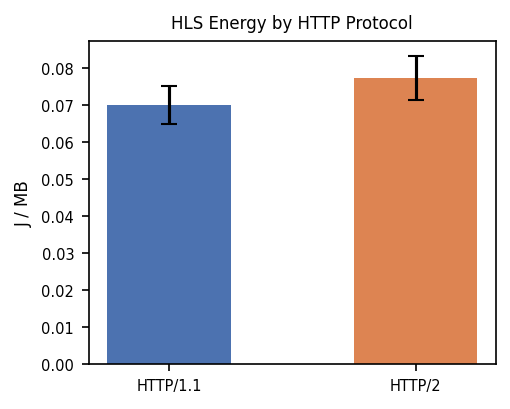
\includegraphics[width=\columnwidth]{01_hls_protocol.png}}
\caption{Median client energy per megabyte for HLS delivery over HTTP/1.1 and
HTTP/2. Error bars show median absolute deviation across 5 trials per configuration.
HTTP/2 consumes approximately 11\% more energy on a local network.}
\label{fig:protocol}
\end{figure}

The HTTP/2 overhead is attributable to its mandatory TLS requirement and additional
framing machinery. On a low-latency loopback link where each segment download
completes in well under 100\,ms, the per-connection setup cost (ALPN negotiation,
HTTP/2 settings exchange, HPACK dynamic table initialization) is not amortized over
many concurrent requests as it would be in a browser fetching dozens of assets.
Instead, the overhead is paid once per session but results in slightly elevated CPU
activity during connection establishment.

\subsection{TLS Impact}

Fig.~\ref{fig:tls} isolates the TLS effect within HTTP/1.1, where both plain and
TLS configurations are available. The difference is small: TLS-off averages
0.0706\,J/MB and TLS-on averages 0.0690\,J/MB across the two HTTP/1.1 sub-groups.

\begin{figure}[t]
\centerline{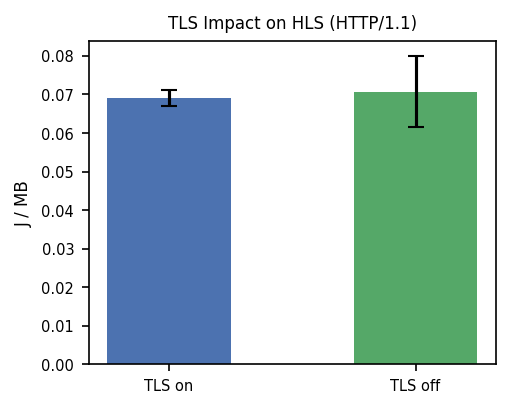
\includegraphics[width=\columnwidth]{02_hls_tls.png}}
\caption{TLS overhead for HLS over HTTP/1.1. The difference between plain and
TLS is within the trial-to-trial variability, indicating TLS imposes negligible
per-megabyte energy cost for long-lived streaming sessions.}
\label{fig:tls}
\end{figure}

The near-zero TLS overhead aligns with expectations for TLS 1.3 on modern hardware:
the handshake completes in one round trip and is amortized over the full 110-second
session. This result supports deploying TLS universally for streaming, as the security
benefit comes at essentially no measurable energy cost.

\subsection{AES-128 Encryption Impact}

Fig.~\ref{fig:drm} compares plain versus AES-128 encrypted HLS segments within
HTTP/1.1. Across both TLS conditions, the encrypted configurations average
0.0695\,J/MB and the plain configurations average 0.0702\,J/MB. The difference of
$<$1\% is well within the MAD of each group.

\begin{figure}[t]
\centerline{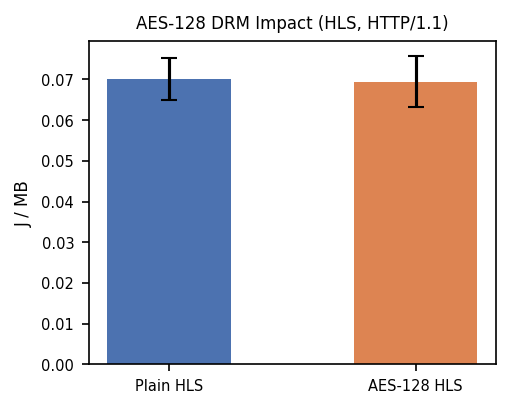
\includegraphics[width=\columnwidth]{04_drm.png}}
\caption{AES-128 segment encryption impact on HLS energy (HTTP/1.1 configurations).
No statistically significant difference is observed between encrypted and plain
segment delivery.}
\label{fig:drm}
\end{figure}

This result is consistent with the availability of hardware AES acceleration on Apple
Silicon: decryption (had it been performed by the emulator) would have added
negligible CPU cycles. Even the key fetch overhead (one additional HTTP GET per
playlist) is absorbed into the total transfer count with no measurable effect.

\subsection{All Configurations}

Fig.~\ref{fig:all} shows all six configurations side by side. The most notable
pattern is the consistent gap between HTTP/2 configurations (right two bars) and
HTTP/1.1 configurations (left four bars), regardless of TLS or encryption setting.
Within HTTP/1.1, the spread across the four sub-configurations is small and overlapping
in MAD, confirming that TLS and AES-128 are not the primary energy drivers.

\begin{figure}[t]
\centerline{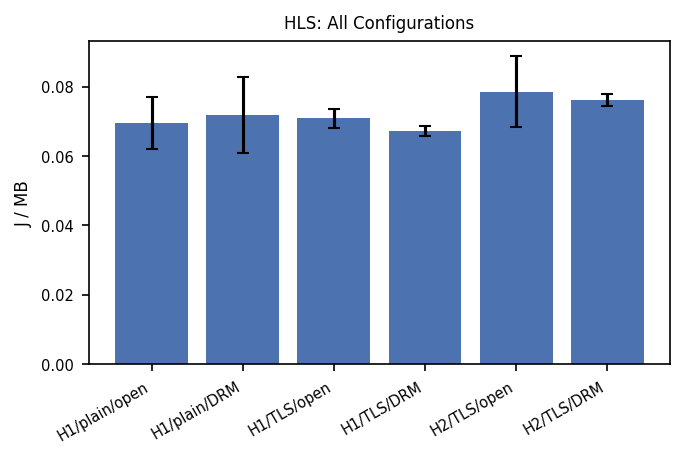
\includegraphics[width=\columnwidth]{03_hls_all_configs.png}}
\caption{All six HLS configurations. HTTP/2 configurations (right) consistently
consume more energy per megabyte than HTTP/1.1 configurations (left), regardless
of TLS or encryption choice.}
\label{fig:all}
\end{figure}

\subsection{Codec and DRM Extension Results}

Table~\ref{tab:codec_drm} reports medians and MAD values from the 50-trial extension.
All runs produced usable power samples ($n_{\text{samples}} \ge 8$), so no row was dropped.

\input{../../../analysis/tables/codec_drm_table.tex}

\subsubsection{Bulk Container Comparison}

Fig.~\ref{fig:codec_bulk} shows median J/MB for rate-limited bulk transfer. MP4 is lowest
(0.1047 J/MB), AV1-MP4 is close (0.1220 J/MB), and MKV is highest (0.1359 J/MB).

\begin{figure}[t]
\centerline{\includegraphics[width=\columnwidth]{../../../analysis/plots/codec_drm_01_codec_bulk.png}}
\caption{Rate-limited bulk transfer energy by container or codec format. Error bars are
MAD across five trials.}
\label{fig:codec_bulk}
\end{figure}

The differences are modest and likely come from a mix of file size, parser overhead, and
short trial duration sensitivity. This is expected because the same host performs both
serving and receiving, and network variability is minimal.

\subsubsection{HLS Codec Comparison}

Fig.~\ref{fig:codec_hls_ext} shows AV1/fMP4 HLS at 0.9554 J/MB versus H.264/TS HLS at
1.1922 J/MB.

\begin{figure}[t]
\centerline{\includegraphics[width=\columnwidth]{../../../analysis/plots/codec_drm_02_codec_hls.png}}
\caption{HLS codec energy comparison between H.264/TS and AV1/fMP4.}
\label{fig:codec_hls_ext}
\end{figure}

The simple explanation is transfer efficiency. The AV1 run moved fewer bytes and completed
faster in this setup, so total joules per megabyte decreased despite codec complexity.

\subsubsection{DRM Scheme Comparison}

Fig.~\ref{fig:drm_ext} compares plaintext, key-fetch-only, and decrypting DRM schemes.
Median values range from 0.5865 to 1.2855 J/MB, with noticeable spread in the plaintext
baseline.

\begin{figure}[t]
\centerline{\includegraphics[width=\columnwidth]{../../../analysis/plots/codec_drm_03_drm_overhead.png}}
\caption{Energy by DRM scheme for HLS with fixed content and HTTP/1.1.}
\label{fig:drm_ext}
\end{figure}

Across decrypting schemes, values are relatively close. This indicates that cipher mode
choice is a second-order effect compared with delivery pacing and background system noise.
In other words, fetching and playing the stream dominates energy more than CBC versus CTR
for this workload scale.

\subsubsection{Decrypt CPU Time}

Fig.~\ref{fig:drm_cpu_ext} reports median decrypt wall-time per stream. AES-128-decrypt and
CBCS are near 333 ms, while CENC is near 356 ms.

\begin{figure}[t]
\centerline{\includegraphics[width=\columnwidth]{../../../analysis/plots/codec_drm_04_decrypt_cpu.png}}
\caption{Measured decrypt CPU wall-time by scheme. Differences are small across cipher
modes for this segment size and trial duration.}
\label{fig:drm_cpu_ext}
\end{figure}

The straightforward interpretation is that all three modes execute similar block-level work
over the same byte volume, so CPU-time differences stay small.


\section{Discussion}

\subsection{Why HTTP/2 Costs More Energy for HLS}

The conventional motivation for deploying HTTP/2 is to reduce page load time by
multiplexing many concurrent requests. A browser loading a webpage with 50 assets
benefits substantially from HTTP/2's single-connection multiplexing. An HLS player,
by contrast, makes requests sequentially: it must receive and buffer one segment before
knowing the timing for the next. The multiplexing advantage is effectively zero for
this access pattern.

What HTTP/2 does add is framing overhead: each request and response body is
transmitted as a sequence of DATA frames with headers in binary HPACK-encoded HEADERS
frames. On a loopback interface where the network is not the bottleneck, the CPU cost
of this additional encoding and the TLS mandatory requirement show up as measurable
energy. For real-world deployments over high-latency wide-area links, HTTP/2's reduced
round-trip count may more than compensate for this overhead. Our loopback results
isolate the pure protocol overhead and indicate that HTTP/2 is not inherently
energy-free.

\subsection{Implications for Content Delivery}

Two practical insights follow from these results:

\textit{First}, operators considering a mandatory HTTP/2 migration for HLS delivery
should account for client energy. At 0.0774\,J/MB versus 0.0699\,J/MB, the difference
is 10.7\%. For a two-hour 1080p stream at 4\,Mbps ($\approx$3.6\,GB), this translates
to approximately 27\,J of additional client energy, or about 2\% of a typical laptop
battery. Across millions of concurrent streams, the aggregate effect is nontrivial.

\textit{Second}, content providers can enable AES-128 segment encryption at no
measurable energy cost on modern client hardware. This has direct policy implications:
providers who have delayed enabling HLS encryption due to concerns about client
battery life can do so without penalty.

\subsection{Limitations}

Several limitations constrain the generalizability of these results.

\textbf{Loopback-only testbed.} All transfers ran over \texttt{localhost}. In a real
network, HTTP/2's reduction of round trips and TCP connections may reduce total
transfer time and thus lower energy per megabyte below the HTTP/1.1 baseline. Our
results represent a best case for HTTP/1.1 and a worst case for HTTP/2's overhead.

\textbf{No idle correction.} The powermetrics idle baseline was collected during
session startup when background OS activity elevated measured power. We use raw energy
rather than corrected energy. This means absolute J/MB values include idle CPU power
and should not be interpreted as the incremental energy attributable to streaming
alone. Relative comparisons across configurations remain valid because all trials
share the same background conditions.

\textbf{macOS only.} The powermetrics approach is macOS-specific. Linux clients would
use RAPL counters, which provide per-domain (CPU package, DRAM, uncore) energy
attribution not available through powermetrics. Replicating this study on Linux would
enable finer-grained measurement.

\textbf{Single client platform.} Apple M-series hardware has efficient AES acceleration
and a sophisticated power management system. Results may differ on x86 laptops, mobile
ARM devices, or embedded players with less capable hardware AES support.

\textbf{Bulk downloads not measurable.} Short bulk file transfers ($<$0.5\,s) fell
below the powermetrics sampling floor and produced zero energy samples. We therefore
report only HLS results in this paper. Future work using a higher-frequency measurement
approach (e.g., external power meters or RAPL on Linux) could capture bulk transfer
energy.

\textbf{DRM implementation is an approximation.} The CENC and CBCS paths model cipher
mode cost in software but do not implement a full commercial license workflow or hardware
trusted execution path. The results should be interpreted as comparative crypto workload
cost, not a full platform DRM certification result.

\subsection{Future Work}

Repeating this experiment over a real wide-area network would reveal how propagation
delay and congestion shift the HTTP/1.1 vs. HTTP/2 trade-off. Adding HTTP/3 (QUIC)
requires a curl build with QUIC support (the system curl on macOS uses LibreSSL, which
lacks it), and would complete the protocol evolution comparison. A parallel server-side
energy measurement using RAPL would quantify whether HTTP/2's connection consolidation
reduces server energy enough to offset the client overhead.

\subsection{Final Takeaways for Deployment Decisions}

The combined results suggest a practical rule: optimize delivery path first, then optimize
security implementation details. In this study, changes in delivery mode and stream format
shifted J/MB more than changes in cipher mode.

\textbf{When to prioritize energy savings.} If a service streams mostly long-form video on
stable networks, and user battery life is a key product metric, companies should prefer the
lowest-energy delivery stack validated on their own clients. In our environment, HTTP/1.1
with efficient media packaging reduced energy versus HTTP/2 for sequential HLS traffic.
For this case, reducing transferred bytes and avoiding unnecessary protocol overhead gives
the largest return.

\textbf{When stronger DRM is worth the energy cost.} If business requirements include studio
licensing, premium release windows, or regional contractual obligations, using Widevine or
equivalent DRM is often mandatory regardless of small client energy overhead. In those cases,
the correct question is not whether DRM is free, but whether the added energy is acceptable
relative to content-value protection and compliance risk. For most premium catalogs, the
business penalty of weak protection is much larger than the measured per-stream energy delta.

\textbf{A simple decision framework.} Teams can evaluate four factors jointly:
\begin{enumerate}
  \item \textit{Content risk}: premium early-release content and high piracy risk favor full
    DRM (for example, Widevine L1 on supported devices).
  \item \textit{Device profile}: battery-constrained mobile audiences increase the importance
    of low J/MB delivery paths.
  \item \textit{Network reality}: if real WAN latency is high, HTTP/2 or HTTP/3 may recover
    enough wall-clock time to offset protocol overhead.
  \item \textit{Regulatory and contractual constraints}: partner requirements can hard-gate the
    feasible security options.
\end{enumerate}

\textbf{Recommended default policy.} Use strong DRM when required by content agreements, then
minimize energy inside that constraint by tuning encoding ladders, segment duration, caching,
and protocol selection per device class. For non-premium content without strict licensing,
lighter protection may be acceptable, and delivery efficiency should dominate the design.


\section{Conclusion}

We measured client-side streaming energy with two controlled suites on macOS. In the first
suite (30 trials), HTTP/2 consumed more energy per megabyte than HTTP/1.1 for sequential
HLS requests, while TLS and AES-128 toggles were within small variability bands. In the
second suite (50 trials), AV1/fMP4 HLS showed lower J/MB than H.264/TS HLS in our setup,
and DRM decryption-mode differences were smaller than delivery-mode differences.

The central practical conclusion is simple. For this local, low-latency environment,
delivery pattern and transfer duration are the main energy drivers. Security features and
cipher-mode choice contribute less to total client energy than protocol and media-pipeline
structure.


\section*{Acknowledgment}

We thank the teaching staff of Energy Efficient Computing for providing us with
great feedback on the research proposal and key insights into energy consumption
throughout the semester.


\begin{thebibliography}{00}

\bibitem{b_sandvine}
Sandvine, ``The Global Internet Phenomena Report,'' Sandvine Inc., Waterloo, Canada,
2023. [Online]. Available: https://www.sandvine.com/global-internet-phenomena-report

\bibitem{b_cisco}
Cisco Systems, ``Cisco Annual Internet Report (2018--2023) White Paper,'' Cisco Systems
Inc., San Jose, CA, 2020. [Online]. Available:
https://www.cisco.com/c/en/us/solutions/collateral/executive-perspectives/annual-internet-report/white-paper-c11-741490.html

\bibitem{b_hls_rfc}
R. Pantos and W. May, ``HTTP Live Streaming,'' RFC 8216, Internet Engineering Task Force,
Aug. 2017. [Online]. Available: https://www.rfc-editor.org/rfc/rfc8216

\bibitem{b_http11}
R. Fielding and J. Reschke, ``Hypertext Transfer Protocol (HTTP/1.1): Message Syntax and
Routing,'' RFC 7230, Internet Engineering Task Force, Jun. 2014. [Online]. Available:
https://www.rfc-editor.org/rfc/rfc7230

\bibitem{b_http2}
M. Belshe, R. Peon, and M. Thomson, ``Hypertext Transfer Protocol Version 2 (HTTP/2),''
RFC 9113, Internet Engineering Task Force, Jun. 2022. [Online]. Available:
https://www.rfc-editor.org/rfc/rfc9113

\bibitem{b_tls}
E. Rescorla, ``The Transport Layer Security (TLS) Protocol Version 1.3,'' RFC 8446,
Internet Engineering Task Force, Aug. 2018. [Online]. Available:
https://www.rfc-editor.org/rfc/rfc8446

\bibitem{b_aesni}
S. Gueron, ``Intel Advanced Encryption Standard (AES) New Instructions Set,'' Intel
Corporation, Rev. 3.01, Sep. 2012. [Online]. Available:
https://www.intel.com/content/dam/doc/white-paper/advanced-encryption-standard-new-instructions-set-paper.pdf

\bibitem{b_rapl}
N. H. Khan, A. Marathe, J. Moore, M. Schulz, and B. R. de Supinski, ``RAPL in action:
Experiences in using RAPL for power measurements,'' \textit{ACM Trans. Model. Perform.
Eval. Comput. Syst.}, vol. 3, no. 2, pp. 1--26, Mar. 2018.

\bibitem{b_powermetrics}
Apple Inc., ``powermetrics(1) Manual Page,'' Apple Developer Documentation, 2023.
[Online]. Available: https://developer.apple.com/documentation

\bibitem{b_http2_perf}
A. Langley \textit{et al.}, ``The QUIC transport protocol: Design and Internet-scale
deployment,'' in \textit{Proc. ACM SIGCOMM}, Los Angeles, CA, Aug. 2017, pp. 183--196.

\end{thebibliography}

\end{document}
